\section{The Word is Silence Expressed}

\emph{The Multiple States of the Being} is \textbf{Rene Guenon}`s fundamental work on metaphysics. In it he explains that ``just as Unity (Being) is nothing but the metaphysical Zero (Non-Being) affirmed, the word is silence expressed." That is, Silence contains within itself the possibility of the Word.

\begin{wrapfigure}{rt}{.16\textwidth}
 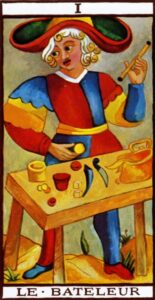
\includegraphics[scale=3]{a20221115TheWordisSilenceExpressed-img001.jpg} 
\end{wrapfigure}

But the Silence is more than the word. The latter is silence expressed, but Silence must needs include as well the inexpressible. Hence, Silence is related to mystery, which refers to something inexpressible, not incomprehensible (which is a common misconception). The implication here is that the understanding of a mystery requires intuition, a direct knowing of the inexpressible; what can be expressed can, on the other hand, be known through discursive thought.

Guenon makes some interesting etymological connections. The Greek \emph{mysterion} derives from \emph{myein} which means ``to be silent". The same root \emph{mu} in Latin is used in \emph{mutus}, ``mute", but more significantly in the word \emph{mythos}, ``myth". So a myth refers to that which is inexpressible, that is, something that can only be expressed indirectly by means of symbolic representations.

In \emph{Meditations on the Tarot}, this Silence is related to concentration without effort. To know this Silence is \emph{to be }this Silence. That is, the discursive mind is quieted of its thoughts, images, desires. This is a concentration, not \emph{of} something, but the effortless concentration of the Silence. We read there:

\begin{quotex}
Concentration \emph{without effort}, which means there is nothing to suppress and where contemplation becomes as natural as breathing and the beating of the heart, is the state of consciousness — of the intellect, the imagination, the feelings, and the will — a state of perfect calm, accompanied by the complete relaxation of the nerves and muscles of the body. It is the deep silence of desires, concerns, imagination, memory, and discursive thought. We would say that the entire being has become like the surface of calm waters reflecting the immense presence of the starry sky and its inexpressible harmony. And the waters are deep, oh how deep! And the silence increases, always increasing, what SILENCE! Its growth takes place in regular waves which pass, one after the other, through your being: one wave of silence followed by another wave of deeper silence, then yet another wave of even deeper silence … Have you ever \emph{drunk the silence}. If so, you know what concentration without effort it.

\end{quotex}
Originally published on 2011-02-11 in medtarot



\flrightit{Posted on 2022-11-15 by Cologero }

\begin{center}* * *\end{center}

\begin{footnotesize}\begin{sffamily}



\texttt{De Bosit on 2022-11-16 at 13:14 said: }

Drinking silence for me was an exercise lying down on my back in bed before going to bed and just trying to quiet the mind. 

But I think the way to actually reflect the starry sky (lets say you work with noisy colleagues and have to do your job) is actually much more beneficial.

You don't realize the „intake`` of information in these quiet moments. But doors open and tunnels are dug deeper and deeper.


\end{sffamily}\end{footnotesize}
